% Created by tikzDevice version 0.12.3.1 on 2021-12-06 11:02:56
% !TEX encoding = UTF-8 Unicode
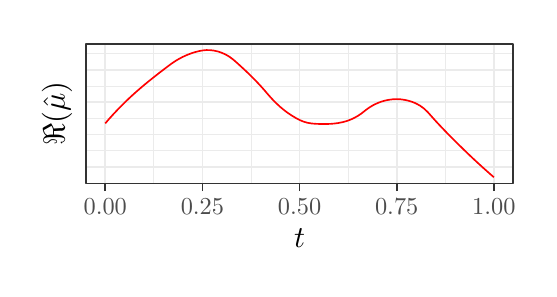
\begin{tikzpicture}[x=1pt,y=1pt]
\definecolor{fillColor}{RGB}{255,255,255}
\begin{scope}
\definecolor{drawColor}{RGB}{255,255,255}
\definecolor{fillColor}{RGB}{255,255,255}

\path[draw=drawColor,line width= 0.6pt,line join=round,line cap=round,fill=fillColor] (  0.00,  0.00) rectangle (180.67, 86.72);
\end{scope}
\begin{scope}
\definecolor{fillColor}{RGB}{255,255,255}

\path[fill=fillColor] ( 20.71, 30.69) rectangle (175.17, 81.22);
\definecolor{drawColor}{gray}{0.92}

\path[draw=drawColor,line width= 0.3pt,line join=round] ( 20.71, 30.90) --
	(175.17, 30.90);

\path[draw=drawColor,line width= 0.3pt,line join=round] ( 20.71, 42.58) --
	(175.17, 42.58);

\path[draw=drawColor,line width= 0.3pt,line join=round] ( 20.71, 54.26) --
	(175.17, 54.26);

\path[draw=drawColor,line width= 0.3pt,line join=round] ( 20.71, 65.94) --
	(175.17, 65.94);

\path[draw=drawColor,line width= 0.3pt,line join=round] ( 20.71, 77.62) --
	(175.17, 77.62);

\path[draw=drawColor,line width= 0.3pt,line join=round] ( 45.29, 30.69) --
	( 45.29, 81.22);

\path[draw=drawColor,line width= 0.3pt,line join=round] ( 80.39, 30.69) --
	( 80.39, 81.22);

\path[draw=drawColor,line width= 0.3pt,line join=round] (115.50, 30.69) --
	(115.50, 81.22);

\path[draw=drawColor,line width= 0.3pt,line join=round] (150.60, 30.69) --
	(150.60, 81.22);

\path[draw=drawColor,line width= 0.6pt,line join=round] ( 20.71, 36.74) --
	(175.17, 36.74);

\path[draw=drawColor,line width= 0.6pt,line join=round] ( 20.71, 48.42) --
	(175.17, 48.42);

\path[draw=drawColor,line width= 0.6pt,line join=round] ( 20.71, 60.10) --
	(175.17, 60.10);

\path[draw=drawColor,line width= 0.6pt,line join=round] ( 20.71, 71.78) --
	(175.17, 71.78);

\path[draw=drawColor,line width= 0.6pt,line join=round] ( 27.74, 30.69) --
	( 27.74, 81.22);

\path[draw=drawColor,line width= 0.6pt,line join=round] ( 62.84, 30.69) --
	( 62.84, 81.22);

\path[draw=drawColor,line width= 0.6pt,line join=round] ( 97.94, 30.69) --
	( 97.94, 81.22);

\path[draw=drawColor,line width= 0.6pt,line join=round] (133.05, 30.69) --
	(133.05, 81.22);

\path[draw=drawColor,line width= 0.6pt,line join=round] (168.15, 30.69) --
	(168.15, 81.22);
\definecolor{drawColor}{RGB}{255,0,0}

\path[draw=drawColor,line width= 0.6pt,line join=round] ( 27.74, 52.44) --
	( 29.14, 54.06) --
	( 30.54, 55.62) --
	( 31.95, 57.12) --
	( 33.35, 58.57) --
	( 34.76, 59.97) --
	( 36.16, 61.32) --
	( 37.56, 62.62) --
	( 38.97, 63.88) --
	( 40.37, 65.10) --
	( 41.78, 66.29) --
	( 43.18, 67.45) --
	( 44.59, 68.58) --
	( 45.99, 69.69) --
	( 47.39, 70.79) --
	( 48.80, 71.86) --
	( 50.20, 72.93) --
	( 51.61, 73.98) --
	( 53.01, 74.93) --
	( 54.41, 75.76) --
	( 55.82, 76.50) --
	( 57.22, 77.13) --
	( 58.63, 77.68) --
	( 60.03, 78.14) --
	( 61.44, 78.51) --
	( 62.84, 78.78) --
	( 64.24, 78.93) --
	( 65.65, 78.90) --
	( 67.05, 78.73) --
	( 68.46, 78.41) --
	( 69.86, 77.93) --
	( 71.27, 77.30) --
	( 72.67, 76.47) --
	( 74.07, 75.42) --
	( 75.48, 74.18) --
	( 76.88, 72.90) --
	( 78.29, 71.60) --
	( 79.69, 70.26) --
	( 81.09, 68.87) --
	( 82.50, 67.43) --
	( 83.90, 65.93) --
	( 85.31, 64.35) --
	( 86.71, 62.70) --
	( 88.12, 61.14) --
	( 89.52, 59.72) --
	( 90.92, 58.42) --
	( 92.33, 57.25) --
	( 93.73, 56.20) --
	( 95.14, 55.26) --
	( 96.54, 54.41) --
	( 97.94, 53.67) --
	( 99.35, 53.08) --
	(100.75, 52.67) --
	(102.16, 52.42) --
	(103.56, 52.29) --
	(104.97, 52.23) --
	(106.37, 52.21) --
	(107.77, 52.22) --
	(109.18, 52.26) --
	(110.58, 52.38) --
	(111.99, 52.57) --
	(113.39, 52.85) --
	(114.79, 53.22) --
	(116.20, 53.72) --
	(117.60, 54.35) --
	(119.01, 55.14) --
	(120.41, 56.09) --
	(121.82, 57.21) --
	(123.22, 58.22) --
	(124.62, 59.05) --
	(126.03, 59.73) --
	(127.43, 60.27) --
	(128.84, 60.68) --
	(130.24, 60.96) --
	(131.65, 61.14) --
	(133.05, 61.20) --
	(134.45, 61.14) --
	(135.86, 60.94) --
	(137.26, 60.63) --
	(138.67, 60.20) --
	(140.07, 59.61) --
	(141.47, 58.84) --
	(142.88, 57.82) --
	(144.28, 56.49) --
	(145.69, 54.90) --
	(147.09, 53.34) --
	(148.50, 51.82) --
	(149.90, 50.35) --
	(151.30, 48.90) --
	(152.71, 47.48) --
	(154.11, 46.07) --
	(155.52, 44.68) --
	(156.92, 43.30) --
	(158.32, 41.94) --
	(159.73, 40.60) --
	(161.13, 39.28) --
	(162.54, 37.98) --
	(163.94, 36.70) --
	(165.35, 35.44) --
	(166.75, 34.20) --
	(168.15, 32.98);
\definecolor{drawColor}{gray}{0.20}

\path[draw=drawColor,line width= 0.6pt,line join=round,line cap=round] ( 20.71, 30.69) rectangle (175.17, 81.22);
\end{scope}
\begin{scope}
\definecolor{drawColor}{gray}{0.20}

\path[draw=drawColor,line width= 0.6pt,line join=round] ( 27.74, 27.94) --
	( 27.74, 30.69);

\path[draw=drawColor,line width= 0.6pt,line join=round] ( 62.84, 27.94) --
	( 62.84, 30.69);

\path[draw=drawColor,line width= 0.6pt,line join=round] ( 97.94, 27.94) --
	( 97.94, 30.69);

\path[draw=drawColor,line width= 0.6pt,line join=round] (133.05, 27.94) --
	(133.05, 30.69);

\path[draw=drawColor,line width= 0.6pt,line join=round] (168.15, 27.94) --
	(168.15, 30.69);
\end{scope}
\begin{scope}
\definecolor{drawColor}{gray}{0.30}

\node[text=drawColor,anchor=base,inner sep=0pt, outer sep=0pt, scale=  0.88] at ( 27.74, 19.68) {0.00};

\node[text=drawColor,anchor=base,inner sep=0pt, outer sep=0pt, scale=  0.88] at ( 62.84, 19.68) {0.25};

\node[text=drawColor,anchor=base,inner sep=0pt, outer sep=0pt, scale=  0.88] at ( 97.94, 19.68) {0.50};

\node[text=drawColor,anchor=base,inner sep=0pt, outer sep=0pt, scale=  0.88] at (133.05, 19.68) {0.75};

\node[text=drawColor,anchor=base,inner sep=0pt, outer sep=0pt, scale=  0.88] at (168.15, 19.68) {1.00};
\end{scope}
\begin{scope}
\definecolor{drawColor}{RGB}{0,0,0}

\node[text=drawColor,anchor=base,inner sep=0pt, outer sep=0pt, scale=  1.10] at ( 97.94,  7.64) {$t$};
\end{scope}
\begin{scope}
\definecolor{drawColor}{RGB}{0,0,0}

\node[text=drawColor,rotate= 90.00,anchor=base,inner sep=0pt, outer sep=0pt, scale=  1.10] at ( 13.08, 55.95) {$\Re(\hat\mu)$};
\end{scope}
\end{tikzpicture}
